\chapter{Graphs That Describe the World}
\label{chap:graphs-describe-the-world}

Before we can talk about WARP graphs, or rewrite rules, or worldlines, or any of the wild machinery that shows up later in this book, we need to agree on one simple thing:

\textbf{We need a language for structure.}

I don't mean code. I don't mean data types, or UML, or "software architecture" diagrams that get drawn on a whiteboard once and then immediately drift out of date. I'm not talking about features, or Jira tickets, or boxes-and-arrows in a slide deck that are designed to impress management rather than describe reality.

I am talking about structure itself. The quiet skeleton underneath everything else.

\textbf{Graph theory is that language.}

Not because it's academic. Not because it's fashionable in certain circles of functional programming or category theory. But because when you strip away the noise—the variable names, the frameworks, the implementation details, the tribal preferences of syntax—you are left with something universal:

\textbf{Things that exist, and the ways they connect.}

\textit{That} is a graph.

And once you learn to see the world as graphs, everything in software starts behaving... differently. Cleaner. More legible. More honest. You stop seeing objects and start seeing relationships. You stop seeing "data" and start seeing topology.

Let's start small.

\section{Nodes and Edges: The Simplest Possible Universe}
\label{sec:nodes-and-edges}

A graph, in its most elemental form, is just two things:
\begin{enumerate}
    \item \textbf{Nodes}: The "things" or entities in your system.
    \item \textbf{Edges}: The relationships or connections between those things.
\end{enumerate}

That is it. The entire universe of structure is built from these atoms. You could draw one right now with two dots and a line.

\begin{figure}[h]
    \centering
    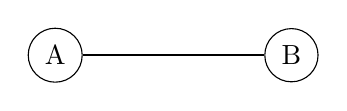
\begin{tikzpicture}[node distance=3cm, auto]
        \node (A) [draw, circle] {A};
        \node (B) [draw, circle, right of=A] {B};
        \draw[thick] (A) -- (B);
    \end{tikzpicture}
    \caption{The fundamental atom of structure: A relation between two entities.}
    \label{fig:simple_graph}
\end{figure}

Congratulations, you have just built a model of:
\begin{itemize}
    \item A marriage.
    \item A network link between two servers.
    \item A function call.
    \item A collision event between a player and a wall.
    \item A software dependency.
    \item A synapse firing between neurons.
    \item A file importing another file.
    \item A job depending on a previous job.
    \item A door connecting two rooms in a level.
    \item A row in a truth table.
    \item A web of trust.
    \item An electric circuit.
    \item A Git commit referencing its parent.
    \item Or the center of a galaxy tugging at a star.
\end{itemize}

That is the magic. Graphs are agnostic. They don't care what domain you live in. They don't care if you are modeling subatomic particles or social networks. They are the universal bookkeeping system for relationships. And relationships are everywhere.

\section{Directed vs. Undirected: The Nature of the Bond}
\label{sec:directed-vs-undirected}

Not all connections are created equal. Some relationships have a definitive flow. These are \textbf{Directed} graphs.

\[ A \rightarrow B \]

This arrow represents an asymmetry in the relationship:
\begin{itemize}
    \item "A depends on B" (but B might not know A exists).
    \item "This task must run \textit{before} that one."
    \item "This event \textit{causes} that event."
    \item "This asset includes that file."
    \item "This commit comes \textit{after} that commit."
\end{itemize}

Other relationships are symmetric. These are \textbf{Undirected} graphs.

\[ A \text{ --- } B \]

This line represents mutuality:
\begin{itemize}
    \item "These two objects collided."
    \item "These systems communicate via a peer-to-peer link."
    \item "These tasks share state."
\end{itemize}

Directionality matters because it captures the difference between hierarchy and partnership—the difference between "I need you" and "we are in this together." Most real-world systems are a complex mix of both.

\section{Cycles \& Acyclicity: Flows vs. Loops}
\label{sec:cycles-acyclicity}

The shape of the path through the graph defines the behavior of the system.

\textbf{An Acyclic Graph (DAG)} moves in one direction. It has a beginning and an end.
\[ A \rightarrow B \rightarrow C \]
This is the shape of build systems, data pipelines, compilers, and most of Git history (ignoring merge conflicts). It represents progress, causality, and time.

\textbf{A Cycle} loops back on itself.
\[ A \rightarrow B \rightarrow C \rightarrow A \]
This is the shape of feedback loops, game loops, simulation ticks, control systems, UI rendering cycles, and agent-based interactions. Cycles aren't "bad." They are how anything dynamic stays alive. A system without cycles is a script; a system with cycles is an engine.

But cycles without rules? That is how a dynamic system becomes chaos. Infinite loops, deadlocks, and race conditions are simply cycles that have lost their governance.

\section{Attributes \& Labels: A Tiny Universe}
\label{sec:attributes-labels}

Nodes and edges are rarely empty containers. In any useful model, they hold information.

\[ [\text{Player}] \xrightarrow{\text{collides at } t=1.45s} [\text{Wall}] \]

This turns a raw graph into a semantic model. Nodes gain hit points, identifiers, and types. Edges gain timestamps, thresholds, probabilities, and priorities.

\begin{figure}[h]
    \centering
    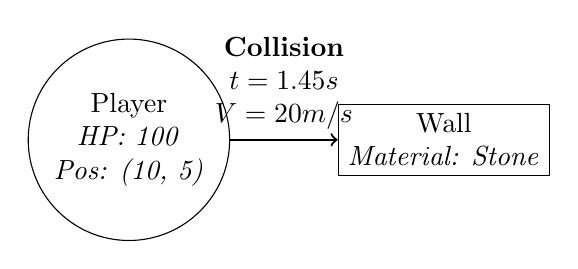
\begin{tikzpicture}[node distance=4cm, auto]
        \node (P) [draw, circle, align=center] {Player \\ \textit{HP: 100} \\ \textit{Pos: (10, 5)}};
        \node (W) [draw, rectangle, right of=P, align=center] {Wall \\ \textit{Material: Stone}};
        
        \draw[->, thick] (P) -- node[align=center] {\textbf{Collision} \\ $t=1.45s$ \\ $V=20m/s$} (W);
    \end{tikzpicture}
    \caption{A labeled graph acts as a semantic model of the world.}
    \label{fig:labeled_graph}
\end{figure}

The key idea is this: \textbf{A graph with labels is a tiny universe.}

It contains entities, relationships, and facts about both. Everything that exists inside a running system—from the values in memory to the packets on the wire—is just a more complicated version of this labeled structure.

\section{The Real Twist: Graphs Describe State}
\label{sec:graphs-describe-state}

Here is where we connect the insights of Chapter 1 to the formalism of Chapter 2.

A graph isn't just a static picture of structure, like a blueprint.

\textbf{\textit{A graph is state.}}

When you load a level, or parse a JSON blob, or build a dependency tree, or initialize a game engine, or sync a distributed store, what you are really doing is building a graph that represents what the world looks like \textit{right now}.

That is the moment when things get interesting. Because if a graph is state...

\textbf{Then a change in state is a change in the graph.}

\[ \text{Old Graph} \xrightarrow{\text{something happens}} \text{New Graph} \]

This is exactly the transition that rewrite rules will formalize in later chapters. But for now, you don't need the math. You just need the intuition:

Graphs are the fundamental structure describing what exists and what depends on what. Everything else—logic, behavior, time—is built on top of that substrate.

\section{The Surprise: You Already Think in Graphs}
\label{sec:you-already-think-graphs}

Most engineers don't realize this, but they are already fluent in this language.
\begin{itemize}
    \item Your \textbf{folder structures} are trees.
    \item Your \textbf{imports and includes} form a directed graph.
    \item Your \textbf{dependency management} is literally resolving a graph.
    \item \textbf{ECS architectures} link entities to components.
    \item \textbf{Behavior trees} in AI are... well, trees.
    \item \textbf{Physics constraint systems} are graphs of rigid bodies and joints.
    \item \textbf{Job schedulers} manage DAGs of tasks.
    \item \textbf{Microservice diagrams} map the topology of a network.
    \item \textbf{Database schemas} define relations (edges) between tables (nodes).
    \item \textbf{Git history} is a Merkle DAG.
    \item \textbf{GPU pipelines} are flow graphs.
    \item \textbf{Syntax trees} drive your compiler.
    \item \textbf{UI widget hierarchies} are the DOM of your application.
\end{itemize}

Every time you say "this thing depends on that thing," or "this must happen before that," or "this triggers that," or "these two systems share data," or "this component talks to that component," or "this structure nests inside that one"—you are speaking graph theory without realizing it.

This chapter isn't trying to teach you something new. It is trying to name something you have been doing your entire career.

\section{The Bridge to What Comes Next}
\label{sec:bridge-next}

Chapter 2 is the broccoli: the clean, simple structure we need to ingest before things get wild. We need this shared language because the logic follows a strict implication chain:

\begin{enumerate}
    \item If \textbf{graphs} describe state...
    \item Then \textbf{sequences of graphs} describe evolution.
\end{enumerate}

And if we can describe evolution, then we can describe everything:
\begin{itemize}
    \item Behavior
    \item Computation
    \item Systems
    \item Transactions
    \item Causality
    \item Worldlines
    \item Counterfactuals
    \item Debugging
    \item Provenance
\end{itemize}

And eventually, this path leads us to MRMW and DPO rewrites.

This is where the book pivots. We started with real-life engineering stories. We moved through flow, structure, and intuition. Now we have the vocabulary we need.

Next up is the big one. The concept that anchors the entire rest of the book. The idea everything else hangs on. The door we have been walking toward since page one:

\textbf{Graphs All the Way Down.}
